\documentclass[18pt]{beamer}
\usepackage[utf8]{inputenc}
\usepackage{templates/mytemplate}
\usepackage{graphicx}
\usepackage{microtype}
\usepackage{listings}
\usepackage{xcolor}
\usepackage{siunitx}
\usepackage{physics}

\hypersetup{colorlinks, linkcolor=black, urlcolor=kit-blue100}
\lstset{
  basicstyle=\ttfamily,
  basicstyle=\footnotesize,
  language=C++,
}

\newcommand\pro{\item[$\oplus$]}
\newcommand\con{\item[$\ominus$]}

\title{Steps towards a Track Quality Indicator from CDC Tracking}
\subtitle{Roadmap from Curler Clone Rejection to a full Quality Indicator}
\author{Michael Eliachevitch}
\date{10 February 2018}
\titleimage{transparent}
\institute{ETP - KIT}

\begin{document}
\selectlanguage{english}

\begin{frame}
  \titlepage
\end{frame}

\begin{frame}
  \frametitle{Reminder: Track Quality Indicator}
  \begin{itemize}
  \item Goal: Track quality estimator module, which generates a single number: quality indicator (QI)
    \begin{itemize}
    \item encodes probability that track is correctly matched
    \item store QI in tracks and give it to analysts\\
      $\rightarrow$ do cuts on QI to get wanted efficiency vs. purity
    \end{itemize}
  \item Quality Estimator trained using MVA-package on features from:
    \begin{itemize}
    \item quality indicators provided by track finders: VXDTF2, \textbf{CDC}, CKF
    \item fitted tracks: track parameters
    \item merger information
    \item \dots
    \end{itemize}
  \item  \href{https://kds.kek.jp/indico/event/26522/session/10/contribution/75/material/slides/0.pdf}{Overview talk} given by Felix Metzner at B2GM and talk on \href{https://indico.desy.de/indico/event/19869/contribution/14/material/slides/0.pdf}{studies of the full track estimator} by Sebastian Racs at tracking meeting last week
  \item \textbf{CDC Track Quality Indicator}: needed for full QI\\
    $\rightarrow$ not implemented yet, will be done by me
  \end{itemize}
\end{frame}

\begin{frame}
  \frametitle{Current Status Quality Estimation in the CDC}
  \begin{itemize}
  \item CDC track finding already has an MVA fake filter: \texttt{TrackRejecter}
  \item calculates weight, which encodes probability that track is not fake (currently means ``less than 80\% CDC hit purity'')
  \item cuts on filter weights below 0.1, otherwise store it in \texttt{CDCTrack}
  \item currently used at the end of \texttt{TFCDC\_SegmentTrackCombiner}, could also be used seperatly with \texttt{TFCDC\_TrackRejecter} module
  \end{itemize}
  \begin{block}{Can the fake rejecter weight be used as the CDC quality indicator?}
    \begin{itemize}
    \item Yes, just needs to be stored in the corresponding \texttt{RecoTrack} object.
    \item Keep the cut?
    \item \textcolor{kit-red100}{Problem:} Does not encode probability if track is clone. But is that needed at reconstruction level? Possible?
    \item Further inputs for final CDC QI?
    \end{itemize}
  \end{block}

\end{frame}

\begin{frame}
  \frametitle{Local CDC Track Finding}
  \begin{itemize}
  \item two track finding algorithms for CDC standalone tracking available:\\
    \begin{itemize}
    \item global track finding with legendre algorithm
    \item local track finding with cellular automaton (CA)
    \end{itemize}
  \item currently, only global track finding used (and CA in segment finder)
  \item full CA track finding implemented by Oliver Frost:
    \begin{itemize}
    \item creates tracks by combining axial-stereo segment pairs
    \item finds single-segment tracks in first superlayer with $> 15$ hits\\
      $\rightarrow$ no $z$-information, need CKF from SVD to CDC
    \item to enable: \lstinline[basicstyle=\ttfamily, language=Python]{add_cdc_track_finding(with_ca=True, ...)}
    \item CA tracking runs after \texttt{SegmentTrackCombiner}\\
      $\rightarrow$ currently no fake filter applied to CA tracks
    \end{itemize}
    \begin{block}{Enabling CA track finding leads to (as shown in the following slides)}
      \begin{itemize}
      \pro slightly higher efficiency
      \con higher clone rate due to curlers, where multiple loop arms are found
      \end{itemize}
    \end{block}
  \end{itemize}
\end{frame}

\begin{frame}
  \frametitle{Rejection of clones from curlers found by CA}
  \begin{itemize}
  \item Idea: An MVA filter can be used to detect clones from curlers
  \item The resulting filter weight can be used for rejecting clones or saved in track (eg. for CDC QI)
  \item Input variables:
    \begin{itemize}
    \item features of the track itself: dangerous, might bias against secondaries
    \item use variable that relates track to other tracks in event
    \end{itemize}
  \item Goal: Reduce clone rate, but don't reduce finding efficiency on secondaries
  \end{itemize}
\end{frame}

\begin{frame}
  \frametitle{MC truth for clone filter: Clone or best match?}
  \begin{itemize}
  \item So far, only MC truth filter implemented
  \item it will be used for MVA training
  \item current truth definition for ``best match'':
    \begin{itemize}
    \item matched track with lowest number of loops until first hit
      (usually 0)
    \item if multiple tracks with same loop number, best match is track with highest number of matched hits
    \item declare all other tracks ``clone''
    \end{itemize}
  \item other ideas for more sophisticated methods welcome
\end{itemize}
\end{frame}

\begin{frame}
  \frametitle{Figures of Merit}
  \begin{itemize}
  \item based on 5000 MC events with phase 3 setup and background overlay from 16th campaign
  \item CDC-only reconstruction without CA, with CA and with CA and clone truth rejection
  \item \textbf{very preliminary}, don't trust exact numbers, mistakes possible \dots
  \end{itemize}
  \begin{columns}
    \begin{column}{0.33\textwidth}
      \includegraphics[width=\textwidth]{figures/ca_findeff.pdf}
    \end{column}
    \begin{column}{0.33\textwidth}
      \includegraphics[width=\textwidth]{figures/ca_clone_rate.pdf}
    \end{column}
    \begin{column}{0.33\textwidth}
      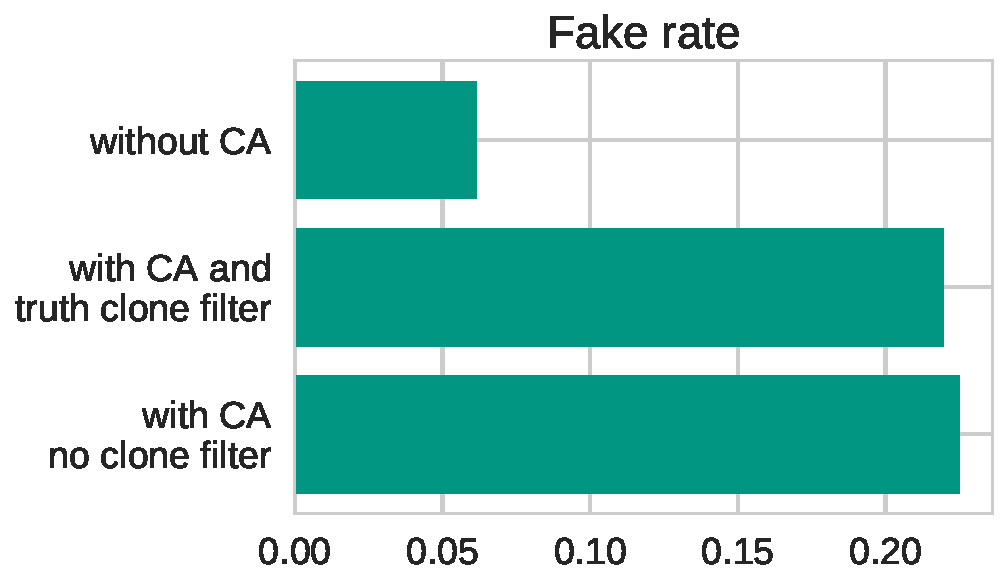
\includegraphics[width=\textwidth]{figures/ca_fake_rate.pdf}
    \end{column}
  \end{columns}
  \begin{itemize}
  \item changes to finding efficiency and clone rate as expected
  \item Why is fake rate so high? Maybe mistake in matching
  \end{itemize}
\end{frame}

\begin{frame}
  \frametitle{Clone distributions}
    \begin{columns}
      \begin{column}{0.65\textwidth}
        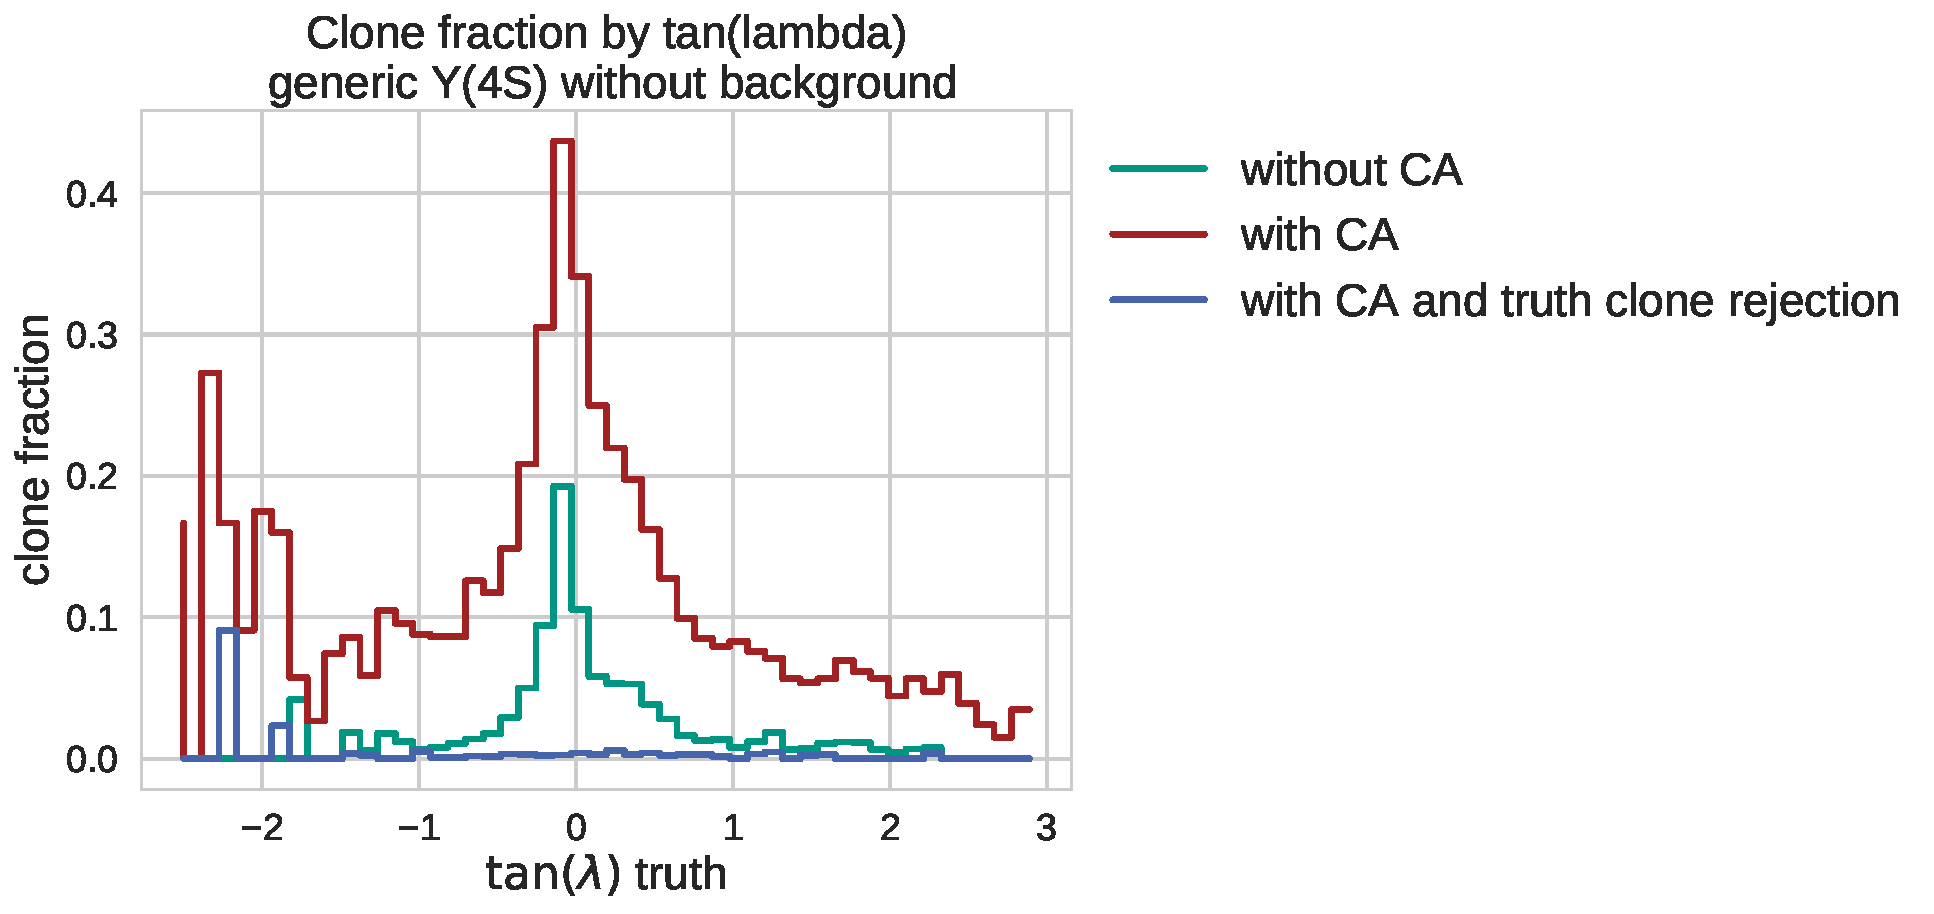
\includegraphics[width=\textwidth]{figures/clone_rate_by_tlambda.pdf}\\
      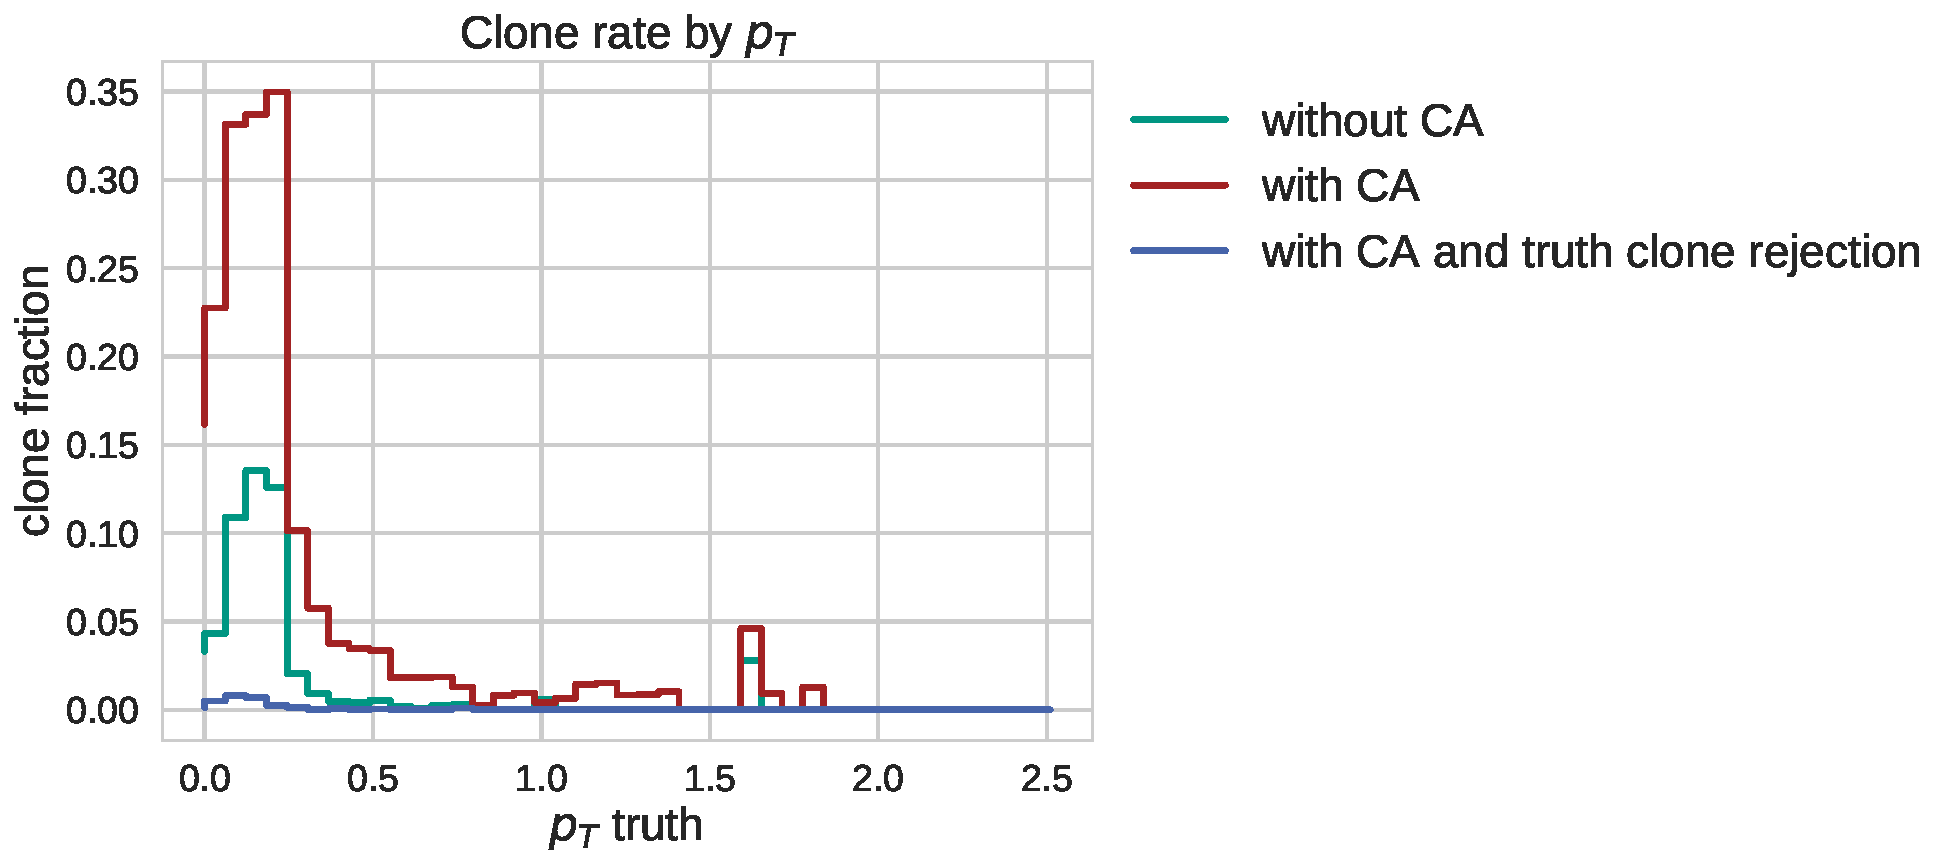
\includegraphics[width=\textwidth]{figures/clone_rate_by_pt.pdf}
    
    \end{column}
    \begin{column}{0.35\textwidth}
      \begin{itemize}
      \item clones come from region around $\tan(\lambda) =\cos(\theta)= 0$
      \item this indicates that they are indeed mostly from curlers
      \end{itemize}
    \end{column}
  \end{columns}
\end{frame}

\begin{frame}
  \frametitle{Conclusion and ToDo's}
  \begin{itemize}
  \item CDC needs to provide its own quality indicator (stored in CDC \texttt{RecoTracks})
  \item some functionality already in \texttt{TrackRejecter} (fake filter) module
  \item further studies CA track finding
    \begin{itemize}
    \item train MVA clone filter (need to select features)
    \item retrain fake filter with CA enables and apply it to CA tracks
    \item check if filter work and if issues with fake rate can be solved
    \end{itemize}
  \item combine individual filters weights into CDC quality estimator module or use them for cuts
  \item train full tracking quality indicator with CDC quality indicator included\\
    (first tests with fake filter weight ongoing)
  \end{itemize}

  
\end{frame}

\appendix
\begin{frame}
  \centering \huge Backup Slides
\end{frame}

\begin{frame}
  \frametitle{Finding efficiency with secondaries}
  \centering
  \includegraphics[width=.8\textwidth]{figures/ca_findeff_w_secondaries.pdf}
\end{frame}

\begin{frame}[allowframebreaks]
  \frametitle{Plots from recording filter output}
  \includegraphics[width=0.4\textwidth]{figures/clone_multiplicities.pdf}\\
  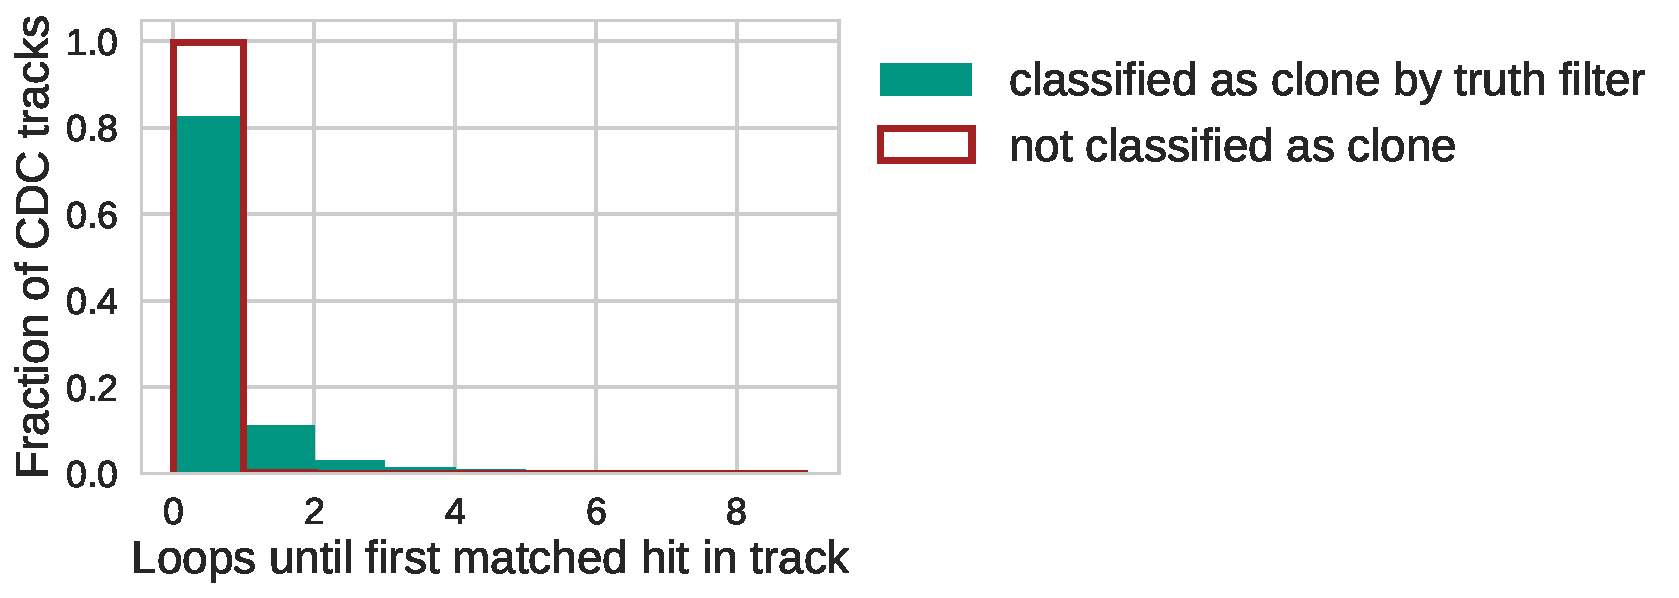
\includegraphics[width=0.7\textwidth]{figures/loop_numbers.pdf}\\
  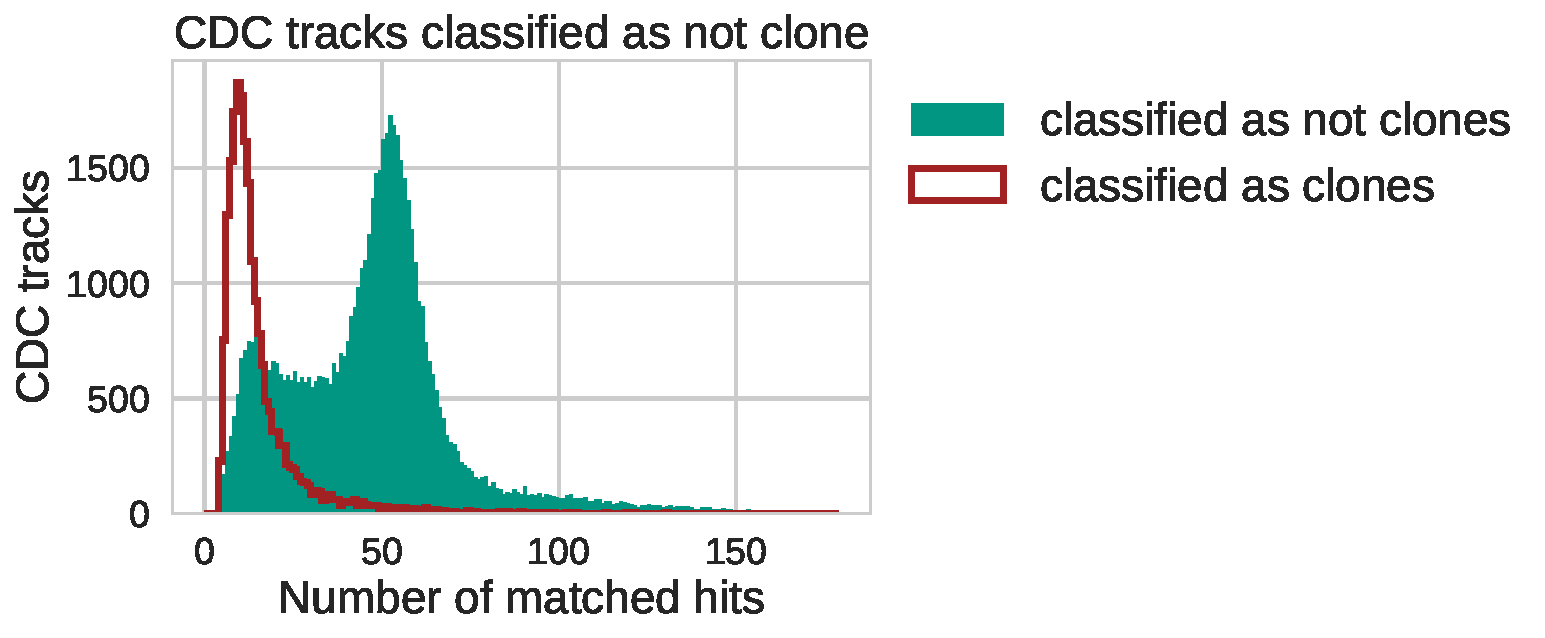
\includegraphics[width=0.7\textwidth]{figures/matched_hits.pdf}\\
\end{frame}

\begin{frame}
  \frametitle{Features currently used for CDC Track Rejecter training}
  As defined in \texttt{tracking/trackFindingCDC/filters/track/BasicTrackVarSet.h}
  \begin{columns}
    \begin{column}{0.5\textwidth}
      \begin{itemize}
      \item \lstinline{size}
      \item \lstinline{pt}
      \item \lstinline{sz_slope}
      \item \lstinline{drift_length_mean}
      \item \lstinline{drift_length_variance}
      \item \lstinline{drift_length_max}
      \item \lstinline{drift_length_min}
      \item \lstinline{drift_length_sum}
      \item \lstinline{adc_mean}
      \item \lstinline{adc_variance}
      \end{itemize}
    \end{column}
    \begin{column}{0.5\textwidth}
      \begin{itemize}

      \item \lstinline{adc_max}
      \item \lstinline{adc_min}
      \item \lstinline{adc_sum}
      \item \lstinline{empty_s_mean}
      \item \lstinline{empty_s_variance}
      \item \lstinline{empty_s_max}
      \item \lstinline{empty_s_min}
      \item \lstinline{empty_s_sum}
      \item \lstinline{has_matching_segment}
      \item \lstinline{s_range}
      \end{itemize}      
    \end{column}
  \end{columns}

\end{frame}

\end{document}

%%% Local Variables:
%%% coding: utf-8
%%% mode: latex
%%% TeX-engine: default
%%% TeX-master: t
%%% End: